\chapter[Data for Evaluation of the Type Stability Approximation Algorithm]{%
  Data for Evaluation of the Type Stability Approximation Algorithm (\secref{sec:approx:eval})}%
\label{app:approx}

The tool implementing the algorithm from~\chapref{chap:approx} has two
technical limitations, in particular:

\begin{itemize}
  \item The tool relies on Julia's type checker, which may fail on some inputs
  for unclear reasons (probably a bug). This rarely happens: for the whole
  corpus it failed on two methods.

  \item Generic methods in Julia, e.g.
  \begin{lstlisting}
    function length(v::Vector{T}) where T
    ...
    end
  \end{lstlisting}
  are represented internally in a different ways than usual methods, e.g.
  \begin{lstlisting}
    function length(v::Vector{T} where T)
    ...
    end
  \end{lstlisting}
  (notice that the \c{where} clause is now inside the parenthesis).
  Currently, the tool is only suited to process the latter form, but not the
  former. In our corpus, an average package contains 14\% of generic methods,
  which our tool currently cannot process. This limitation will be lifted in a
  future version of the tool.
\end{itemize}

\tableref{table:app:eval:abs} contains absolute numbers of the methods processed
by the tool. First four numeric columns: Methods, TyChkErr, Generic, MethodsOK
are related by the following formula:
\begin{equation*}
\text{MethodsOK} = \text{Methods} - \text{TyChkErr} - \text{Generic},
\end{equation*}
which acknowledges the limitations mentioned above. The rest of columns are
divided into two groups, three columns each. In a row of each group the numbers
sum up to the number from MethodsOK in the same row.

\begin{table}%[t]
\caption{Absolute numbers for methods analyzed with the type stability
  approximation algorithm}%
  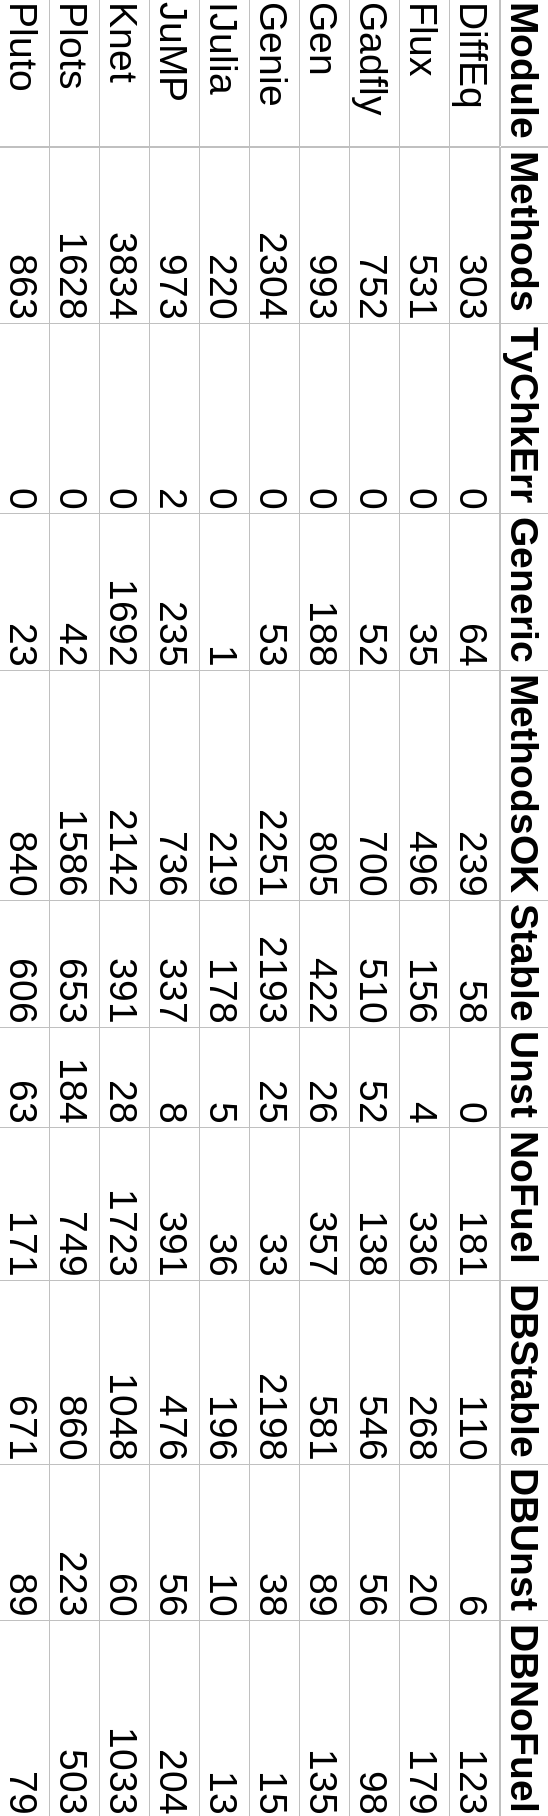
\includegraphics[width=.56\textwidth]
  {figs/sts-eval/table-eval-abs-numbers-rot.png}
\label{table:app:eval:abs}
\end{table}

\begin{table}%[t]
\caption{Percentages for methods analyzed with the type stability
  approximation algorithm. The last two columns are expressed in percentage points.}%
  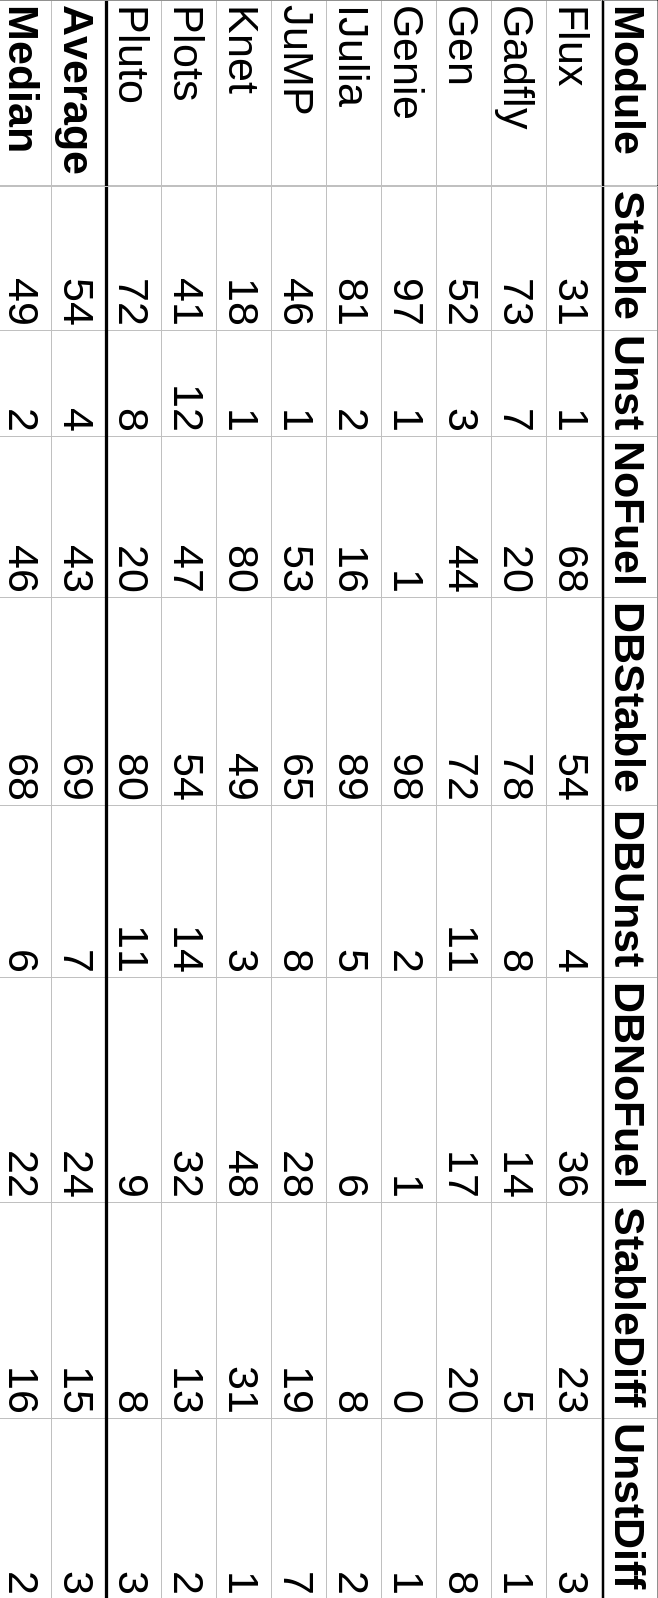
\includegraphics[width=.7\textwidth]
  {figs/sts-eval/table-eval-percent-numbers-rot.png}
%\label{}
\end{table}
